%%%%%%%%%%%%%%%%%%%%%%%%%%%%%%%%%%%%%%%%%
% Dreuw & Deselaer's Poster
% LaTeX Template
% Version 1.0 (11/04/13)
%
% Created by:
% Philippe Dreuw and Thomas Deselaers
% http://www-i6.informatik.rwth-aachen.de/~dreuw/latexbeamerposter.php
% 
% This template has been downloaded from:
% http://www.LaTeXTemplates.com
%
% License:
% CC BY-NC-SA 3.0 (http://creativecommons.org/licenses/by-nc-sa/3.0/)
%
%%%%%%%%%%%%%%%%%%%%%%%%%%%%%%%%%%%%%%%%%

%----------------------------------------------------------------------------------------
%	PACKAGES AND OTHER DOCUMENT CONFIGURATIONS
%----------------------------------------------------------------------------------------

\documentclass[final,hyperref={pdfpagelabels=false}]{beamer}

%\setbeamercolor{block title}{fg=black,bg=orange!70} % Change the block title color
\usepackage{amsmath,amsfonts,amssymb,amsthm,epsfig,epstopdf,titling,url,array}
\newcommand{\bysinfer}{\mathsf{BI}}
\newcommand{\hlg}{\mathsf{H}}
\newcommand{\betafun}{\mathsf{beta}}
%\newcommand{\theHalgorithm}{\arabic{algorithm}}
\theoremstyle{plain}
\newtheorem{thm}{Theorem}[section]
\newtheorem{lem}[thm]{Lemma}
\newtheorem{prop}[thm]{Proposition}
\newtheorem*{cor}{Corollary}

\theoremstyle{definition}
\newtheorem{defn}{Definition}[section]
\newtheorem{conj}{Conjecture}[section]
\newtheorem{exmp}{Example}[section]

\theoremstyle{remark}
\newtheorem*{rem}{Remark}
\newtheorem*{note}{Note}


\usepackage[orientation=landscape,size=custom,width=101.6,height=76.2,scale=1.4]{beamerposter}
%\usepackage[orientation=portrait,size=a0,scale=1.4]{beamerposter} % Use the beamerposter package for laying out the poster with a portrait orientation and an a0 paper size
\usepackage{proof}
%\usetheme{Icy}
\usetheme{I6pd2} % Use the I6pd2 theme supplied with this template

\usepackage[english]{babel} % English language/hyphenation

\usepackage{amsmath,amsthm,amssymb,latexsym} % For including math equations, theorems, symbols, etc

%\usepackage{times}\usefonttheme{professionalfonts}  % Uncomment to use Times as the main font
%\usefonttheme[onlymath]{serif} % Uncomment to use a Serif font within math environments

\boldmath % Use bold for everything within the math environment

\usepackage{booktabs} % Top and bottom rules for tables

\graphicspath{{figures/}} % Location of the graphics files

\usecaptiontemplate{\small\structure{\insertcaptionname~\insertcaptionnumber: }\insertcaption} % A fix for figure numbering

\usepackage{stmaryrd}

%MACROS
\newcommand{\interp}[2]{\llbracket {#2} \rrbracket_{#1}}
\newcommand{\stmod}[1]{\mathfrak{M}[{#1}]}


%----------------------------------------------------------------------------------------
%	TITLE SECTION 
%----------------------------------------------------------------------------------------

\title{\LARGE Tailoring Differentially Private Bayesian Inference to Distance Between Distributions} % Poster title

\author{Mark Bun$^\dag$,
%Imdea Software\\[-3mm]
%\texttt{gjbarthe@gmail.com} \\
%\And 
Gian Pietro Farina$^{*}$,
%University of Dundee\\[-3mm] 
%\texttt{g.p.farina@dundee.ac.uk} \\
%\And
Marco Gaboardi$^{*}$,
%University of Dundee\\[-3mm] 
%\texttt{m.gaboardi@dundee.ac.uk} \\
%\And
Jiawen Liu$^{*}$
%Imdea Software
%\texttt{pierre-yves@strub.nu} \\
}


\institute{$^\dag$Princeton University, $^{*}$University at Buffalo, SUNY} % Institution(s)

%----------------------------------------------------------------------------------------
%	FOOTER TEXT
%----------------------------------------------------------------------------------------

\newcommand{\leftfoot}{Tailoring Differentially Private Bayesian Inference to Distance Between Distributions} % Left footer text

\newcommand{\rightfoot}{mbun@cs.princeton.edu, gaboardi@buffalo.edu} % Right footer text

%----------------------------------------------------------------------------------------

\begin{document}

\addtobeamertemplate{block end}{}{\vspace*{2ex}} % White space under blocks

\begin{frame}[t] % The whole poster is enclosed in one beamer frame

\begin{columns}[t] % The whole poster consists of two major columns, each of which can be subdivided further with another \begin{columns} block - the [t] argument aligns each column's content to the top

\begin{column}{.02\textwidth}\end{column} % Empty spacer column

\begin{column}{.465\textwidth} % The first column

%----------------------------------------------------------------------------------------
%	OBJECTIVES
%----------------------------------------------------------------------------------------

\begin{block}{Objectives}
\noindent Design a mechanism that achieve differential privacy by scaling to a metric between distribution.
\begin{enumerate}
\item A differentially private bayesian mechanism,
\item Calibrating mechanism noise by the same probabilistic distance we want to measure accuracy with.
\item Applying smooth sensitivity in mechanism to achieve better accuracy.
\end{enumerate}

\end{block}

%----------------------------------------------------------------------------------------
%	INTRODUCTION
%----------------------------------------------------------------------------------------
            
\begin{block}{Bayesian Inference Background}
% The first subdivided column within the first main column
% \begin{columns} % Subdivide the first main column
% \begin{column}{.54\textwidth} % The first subdivided column within the first main column
beta
distribution, $\betad(\alpha, \beta)$, with parameters
$\alpha,\beta\in\mathbb{R}^{+}$, and with p.d.f:

\[
  \Pr(\theta)\equiv \frac{\theta^{\alpha} (1- \theta)^{\beta}}{\betaf(\alpha,\beta)}
\]
where $\betaf(\cdot,\cdot)$ is the beta function.
The data $\dataobs$ will be a sequence of $n\in\mathbb{N}$ binary values, that is $\dataobs= (x_1,\dots x_n), x_i\in\{0,1\}$, and the likelihood function is:
\[
  \Pr(\dataobs | \theta)\equiv \theta^{\Delta \alpha}(1-\theta)^{n - \Delta \alpha}
\]
where $\Delta \alpha = \displaystyle\sum_{i=1}^{n}x_i$.
From this it can easily be derived that the posterior distribution is:
\[
  \Pr(\theta|\dataobs)=\betad(\alpha + \Delta \alpha,\beta + n - \Delta \alpha)
\]
\end{block}

%----------------------------------------------------------------------------------------
%	MATERIALS
%----------------------------------------------------------------------------------------

\begin{block}{Differentially private Bayesian inference}
% We are interested in the 
% situation where: we have some  private data $\vec{x}$, some public data
% $\vec{y}$, a set of parameter $\theta$, and a public prior $p(\theta)$
% on $\theta$. We want to compute the public posterior distribution $p(\theta\
% |\ \vec{x}, \vec{y})$ in a differentially private way. This
% corresponds to make sure that
% for given values $\epsilon$ and $\delta$, and for every $\vec{x}$ and $\vec{x'}$ 
% differing in one element we have
Release a private version of posterior distribution $(\tilde\alpha,\tilde\beta)=(\alpha +  \widetilde{\Delta \alpha},\beta + n - \widetilde{\Delta \alpha})$
where $\widetilde{\Delta \alpha}\sim Lap(\Delta \alpha, \frac{2}{\epsilon})$,
and where $Lap(\mu,\nu)$ denotes a Laplace random variable with mean $\mu$ and scale $\nu$.

\end{block}

%----------------------------------------------------------------------------------------
% OUR APPROACH
%----------------------------------------------------------------------------------------


\begin{block}{Our Approach - Exponential Mechanism with Smooth Sensitivity}

define the mechanism $\hexpmech$ which, given in input a
sequence of observations $\dataobs$ and parameters $\epsilon>0$ and
$\delta>0$, produces an element $r$ in $\betaset$ with probability:

\begin{equation*}
\underset{z \thicksim \hexpmech}{\Pr}[z=r] = \frac {exp\big(\frac{-\epsilon\cdot\hellinger(\bysinfer(\dataobs),r)}{2\cdot S(\dataobs)}\big)}
{\displaystyle\sum_{r\in\betaset} exp\Big(\frac{-\epsilon\cdot\hellinger(\bysinfer(\dataobs),r)}{2\cdot S(\dataobs)}\Big)}.
\end{equation*}

The smooth sensitivity is
computed as follows:
\begin{equation}
  \label{eq:smooth}
   S(\dataobs)=\max_{\dataobs' \in \{0,1\}^{n}}\bigg \{\Delta_{l}\bigg (\hellinger(\bysinfer(\dataobs'),\cdot)\bigg )\cdot e^{-\gamma\cdot d(C(\dataobs), C(\dataobs'))}\bigg\},
\end{equation}
where $d$ is the Hamming distance between two datasets,
$\gamma =
\gamma(\epsilon, \delta)$ is a function of $\epsilon$ and $\delta$ to
be determined later, and where $\Delta_{l}\bigg
(\hellinger(\bysinfer(\dataobs'),\cdot)\bigg )$ denotes the local
sensitivity at $\bysinfer(\dataobs')$, or equivalently at $\dataobs'$,
of the scoring function used in our mechanism. That is:
\begin{equation*}
\Delta_{l}\bigg (\hellinger(\bysinfer(\dataobs'),\cdot)\bigg )=\max_{\dataobs'' \in \datauni^n:\adj{\dataobs'}{\dataobs''}, r\in \betaset}\lvert \hellinger(\bysinfer(\dataobs'), r) - \hellinger(\bysinfer(\dataobs''), r)\rvert.
\end{equation*}


\end{block}


\end{column} % End of the first column

\begin{column}{.03\textwidth}\end{column} % Empty spacer column
 
\begin{column}{.465\textwidth} % The second column






\begin{block}{Some Experimental Results}
\begin{figure}[H]
\begin{center}
\centering
  \subfigure[\footnotesize{2-dimensional, data size $\in [100,500]$}]{
    \includegraphics[width=0.328\textwidth]{poster_1.eps}
    \label{fig_1}
  }
  \subfigure[\footnotesize{3-dimensional, data size $\in [100,500]$} ]{
    \includegraphics[width=0.297\textwidth]{poster_2.eps}
  \label{subsubsec_vs_datasize1b}} 
  \subfigure[\footnotesize{4-dimensional, data size $\in [100,600]$}]{
    \includegraphics[width=0.29\textwidth]{poster_3.eps}
    \label{subsubsec_vs_datasize1a}
  }
  \caption{Increasing data size with unit prior $\betad(1,1), \betad(1,1,1)$ and $\betad(1,1,1,1)$, balanced datasets and parameters $\epsilon = 0.8$ and $\delta = 10^{-8}$}
\label{fig_vs_datasize}
\end{center}
\end{figure}

\begin{figure}[H]
\begin{center}
\centering
  \subfigure[2-dimensional]{
    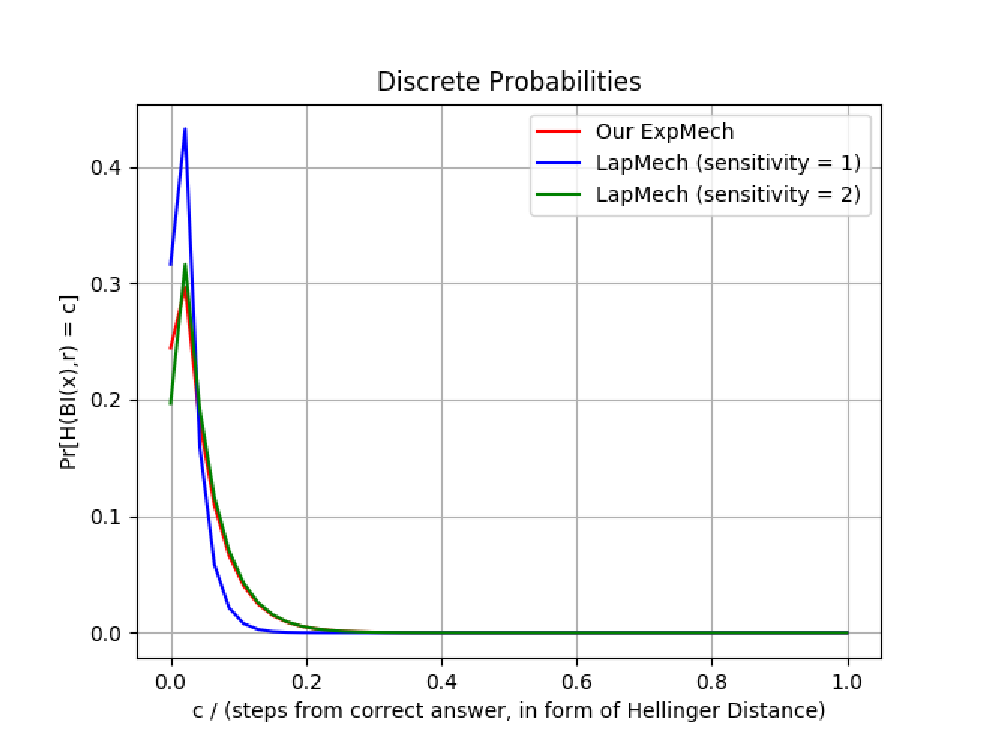
\includegraphics[width=0.31\textwidth]{poster_4.eps}
  \label{subsubsec_vs_datasize1b}}
  \subfigure[3-dimensional]{
    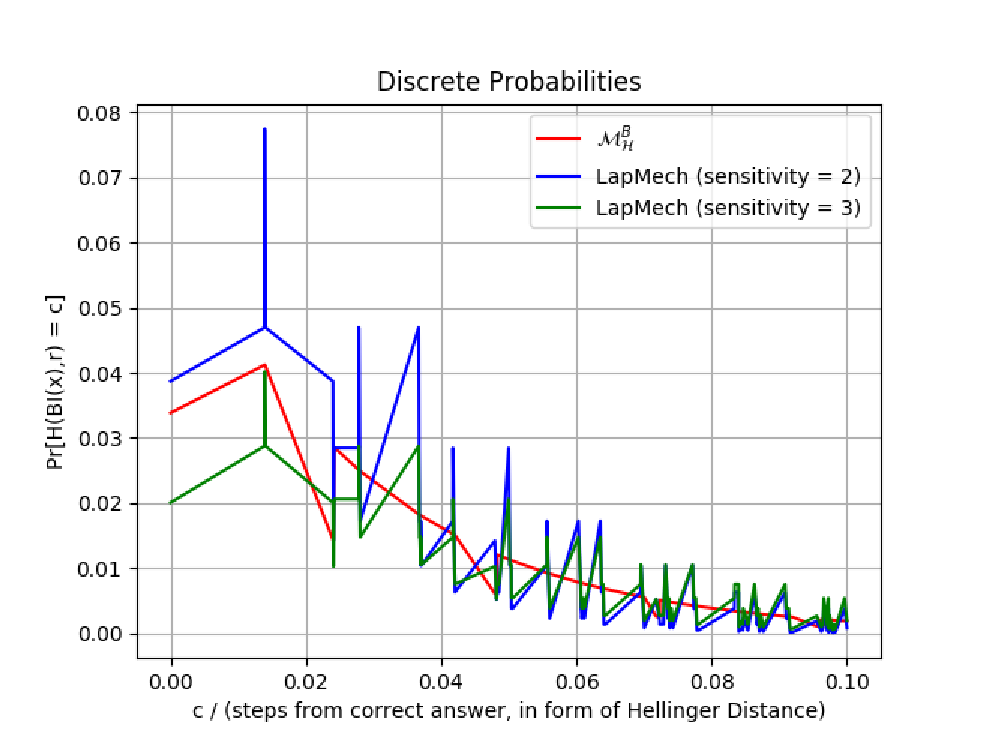
\includegraphics[width=0.31\textwidth]{poster_5.eps}
  \label{subsubsec_vs_datasize1b}} 
  \subfigure[4-dimensional]{
    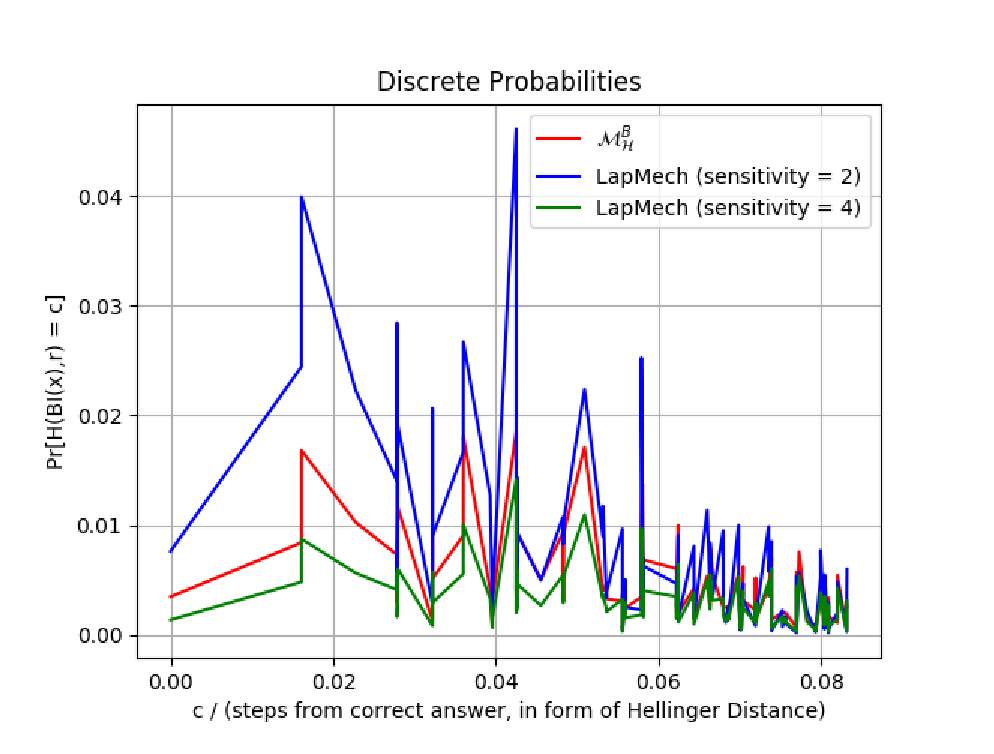
\includegraphics[width=0.31\textwidth]{poster_6.eps}
  \label{subsubsec_vs_datasize1b}} 
\caption{The concrete outputting probabilities under different dimensions with data set of size $600$ ,unit prior $\betad(1,1), \betad(1,1,1)$ and $\betad(1,1,1,1)$, balanced datasets and parameters $\epsilon = 0.8$ and $\delta = 10^{-8}$}
\label{fig_vs_datasize}
\end{center}
\end{figure}

\end{block}


%----------------------------------------------------------------------------------------
% CONCLUSION
%----------------------------------------------------------------------------------------


\begin{block}{Conclusion and Future Work}

\begin{itemize}
  \item Our the probabiliy measure approach outperforms the $\ell_1$-norm approach when the Laplace noise cannot recognize the data to be protected is histogram and data size grow large.

  \item 
  \begin{enumerate}
    \item  The accuracy that we are going to explore next, and in a more principled and formal way.
    
    \item  Experiments have shown that the actual privacy loss
  in the experiments can be smaller than $\epsilon$. This means that we
  could improve accuracy, by adding less noise but still achieve
  $(\epsilon, \delta)$-dp.

    \item The choice of the Hellinger distance might seem quite ad-hoc. Hence, it is worth exploring other distances over distributions. An interesting class of probability metrics is the family of $f$-divergences \cite{CIT-004}.

    \item Other application of our scheme are going to be explored.
  \end{enumerate}
\end{itemize}
%\vspace{8mm}
%\vspace{8mm}
%where we require $t$ and $u$ to have distinct sets of free variables.
\end{block}


%----------------------------------------------------------------------------------------
%	RESULTS
%----------------------------------------------------------------------------------------




%------------------------------------------------

% \begin{block}{Results: Figure}

% \begin{figure}
% \includegraphics[width=0.8\linewidth]{placeholder.jpg}
% \caption{Figure caption}
% \end{figure}

% \end{block}



%----------------------------------------------------------------------------------------
%	REFERENCES
%----------------------------------------------------------------------------------------

\begin{block}{References}
        
%\nocite{*} % Insert publications even if they are not cited in the poster
\small{\bibliographystyle{unsrt}
\bibliography{bayesian}}

\end{block}

%----------------------------------------------------------------------------------------
%	ACKNOWLEDGEMENTS
%----------------------------------------------------------------------------------------

% \begin{block}{Acknowledgments}

% \begin{itemize}
% \item Nam mollis tristique neque eu luctus. Suspendisse rutrum congue nisi sed convallis. Aenean id neque dolor. Pellentesque habitant morbi tristique senectus et netus et malesuada fames ac turpis egestas.
% \end{itemize}

% \end{block}

%----------------------------------------------------------------------------------------
%	CONTACT INFORMATION
%----------------------------------------------------------------------------------------

\setbeamercolor{block title}{fg=black,bg=orange!70} % Change the block title color

% \begin{block}{Contact Information}

% \begin{itemize}
% \item \textbf{Marco Gaboardi}
% \item Web: \href{http://staff.computing.dundee.ac.uk/marcogaboardi/}{http://staff.computing.dundee.ac.uk/marcogaboardi/}
% \item Email: \href{mailto:m.gaboardi@dundee.ac.uk}{m.gaboardi@dundee.ac.uk}
% %\item Phone: +1 617-384-9606
% \end{itemize}

% \end{block}

%----------------------------------------------------------------------------------------

\end{column} % End of the second column

\begin{column}{.015\textwidth}\end{column} % Empty spacer column

\end{columns} % End of all the columns in the poster

\end{frame} % End of the enclosing frame

\end{document}
